\documentclass[a4paper,ngerman]{article}

\usepackage{mathtools}
\usepackage{multicol}
\usepackage[left=2cm,top=1cm,right=2cm,nohead,nofoot]{geometry}

% Switch for 3-column layout
\newif\ifUseColumns

% General includes used by all x3-templates
%
% This file contains preamble settings and packages that are used by in
% all x3-templates
%

% We need this to detect whether or not we're running XeTeX
\usepackage{ifxetex}

% Use UTF-8. XeTeX expects stuff to be in UTF-8, and it
% doesn't like the package to be included.
\ifxetex
	\relax
\else
	\usepackage[utf8]{inputenc}
\fi

% Utility stuff, used, for example, in x3-mmd-compat
% That is why we need to include it here, and not in -begin
\usepackage{etoolbox}


% Make it possible to enable or disable TOC
\newif\ifShowTOC

% Use Helvetica switch
\newif\ifUseHelvetica

% XeLaTex Helvetica Neue Switch
% If you're not using XeTeX, it will just use the regular
% helvetica package.
\newif\ifUseHelveticaNeue

% Language Switch for German (Default is English)
\newif\ifLanguageGerman

% Enable minted (requires -shell-escape option)
\newif\ifUseMinted




% Use Helvetica (Neue)
\UseHelveticaNeuetrue

% Use multicolumn layout
\UseColumnstrue


\raggedcolumns

% ================
% Generic packages
% ================

\usepackage{graphicx}
\usepackage{pdfpages}
\usepackage[hyperfootnotes=false]{hyperref}

\usepackage{float}      % For some reason, figures refuse to show if this package
                        % isn't included.

\usepackage{eurosym}    % The Euro-Symbol (€) for TeX
\usepackage{gensymb}    % Some convenience symbols like \degree
\usepackage{todonotes}  % Todo-notes using \todo
\usepackage{amsmath}    % Additional math symbols



% ================
% Language related
% ================

\ifLanguageGerman % German hyphenation and such
    \usepackage{ngerman}
    \usepackage[ngerman]{babel}

\else % Default is english
    \usepackage[english]{babel}
\fi



% =============
% Fonts related
% =============

% If using XeTeX, use more awesome fonts.
\ifxetex
    % XeTex specific stuff. Only loaded when actually using XeTex,
% by a mechanism in x3-general-begin.

\usepackage{fontspec}
\usepackage{xunicode}
\usepackage{xltxtra}

\setromanfont[Mapping=tex-text]{Garamond}
\setmonofont[Scale=0.85]{Monaco}

\ifUseHelveticaNeue
    \setsansfont[Mapping=tex-text]{Helvetica Neue}
    \renewcommand{\familydefault}{\sfdefault}
\fi

\else
    \ifUseHelveticaNeue
        \UseHelveticatrue
    \fi
\fi

\ifUseHelvetica
    \usepackage{helvet}
    \renewcommand{\familydefault}{\sfdefault}
\else
    \usepackage{kpfonts}    % Kepler fonts for Math
    \usepackage[scaled]{helvet} % Helvetica as sans-serif
    \usepackage{baskervald} % Baskerville clone as serif font
\fi



% =============
% Code listings
% =============

\usepackage{listings}
\ifUseMinted % Minted uses Pygments for highlighting
    \usepackage{minted}
\fi



% ==========================
% Load common layout options
% ==========================


% Contains layout options common to all x3-latex templates

\usepackage{parskip}
\setlength{\parindent}{0cm} % Par-indent is horrible x.x





% Disable section numbering
\setcounter{secnumdepth}{0}

% Begin: Reduce ALL the spacings
\usepackage[compact]{titlesec}
\titlespacing{\section}{0pt}{*0}{*0}
\titlespacing{\subsection}{0pt}{*0}{*0}
\titlespacing{\subsubsection}{0pt}{*0}{*0}

\setlength{\parskip}{0pt}
\setlength{\parsep}{0pt}
\setlength{\headsep}{0pt}
\setlength{\topskip}{0pt}
\setlength{\topmargin}{0pt}
\setlength{\topsep}{0pt}
\setlength{\partopsep}{0pt}
\setlength{\parindent}{0pt}
% End: Reduce ALL the spacings

\usepackage{algpseudocode}

\begin{document}

\ifUseColumns
	\begin{multicols}{3}
\fi







\section{Allgemeines}

\subsection{Good to know}

% arctan2 Definition
\begin{scriptsize}
$ \operatorname{arctan2}(y, x) = $

$ \begin{cases}
\arctan\left(\frac y x\right) & \qquad x > 0 \\
\arctan\left(\frac y x\right) + \pi& \qquad y \ge 0 , x < 0 \\
\arctan\left(\frac y x\right) - \pi& \qquad y < 0 , x < 0 \\
+\frac{\pi}{2} & \qquad y > 0 , x = 0 \\
-\frac{\pi}{2} & \qquad y < 0 , x = 0 \\
\text{undefined} & \qquad y = 0, x = 0
\end{cases} $
\end{scriptsize}

% Sinus-Kosinus Zusammenhang
\[ \sin^2(x) = 1 - \cos^2(x) \]

Bogenmaß vs. Grad \[ \pi rad = 180\degree \]

Euklid. Ursprungsdistanz: \[ r = \sqrt{u^2 + v^2} \]


\subsection{Spezielle Ableitungen}

\[ (\sin(x))' = \cos(x) \]
\[ (\cos(x))' = -\sin(x) \]
\[ (\tan(x))' = \sec^2(x) \]



\subsection{Skalarprodukt und Betrag eines Vektors}

Skalarprodukt:
\[ \vec x\cdot \vec y = \sum_{i=1}^n x_iy_i = {x_1}{y_1}+\dotsb + {x_n}{y_n} \]
\[ \vec x\cdot \vec x = \sum_{i=1}^n x_i = {x_1}^2 +\dotsb + {x_n}^2 \]

Betrag eines Vektors (Länge):
\[ |\vec x| = \sqrt{\vec x \cdot \vec x} \]






\section{Gradienten-Kernel}

\[ G_x = \begin{pmatrix}
-1 & 0 & 1 \\
-2 & 0 & 2 \\
-1 & 0 & 3
\end{pmatrix} \]

\[ G_y = \begin{pmatrix}
-1 & -2 & -1 \\
0 & 0 & 0 \\
1 & 2 & 1
\end{pmatrix} \]

Wert des Gradienten:
\[ G = \sqrt{G_x^2 + G_y^2} \]

Richtung des Gradienten:
\[ \alpha = \operatorname{arctan2}\left(\frac{G_y}{G_x}\right) \]





\columnbreak
\section{Geradengleichung}

\subsection{Steiguns-Abschnitts-Form}

\[ y = mx + b \]


\subsection{Zwei-Punkte-Form}

\begin{scriptsize}
	\[ x(y_j-y_k) + y(x_k-x_j) + y_k \cdot x_j - y_j \cdot x_k = 0 \]
\end{scriptsize}

\subsection{Hesse'sche Normalform}

\[ r = x \cdot \cos \Theta + y \cdot \sin \Theta \]



Achsenabschnittsform

\[ \frac{x}{a} + \frac{y}{b} = 1 \] bzw
\[ Ax + By = 1 = \frac{1}{a}x + \frac{1}{b}y \]


Lineare Funktion $\rightarrow$ Achsenabschnittsform
`b` übernehmen, für `a` gilt:
\[ a = -\frac{b}{m} \]



Achsenabschnittsform $\rightarrow$ Hesse'sche Normalform. Es gilt:
\[ \Theta = \operatorname{arctan2} \left ( \frac{a}{b} \right ) \]
sowie
\[ r = a \cdot \cos \Theta \]






\section{Bilineare Transformation}

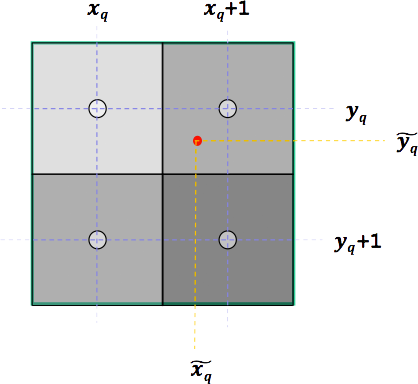
\includegraphics[width=\linewidth]{images/bilinearTransformation.png}


\[
	f(\tilde{x}) = f(x) + (\tilde{x}-x) \cdot \bigg [ f(x+1)-f(x) \bigg ]
\]








\columnbreak
\section{Momentenmethode (Bildschwerpunkt)}

Geometrische Momente eines zweidemnsionalen Objektes der Ordnung $(p,q)$ (nicht translations-invariant, d.h. verändern sich wenn sich das objekt
bewegt):

\[ m_{pq} = \sum_x \sum_y f(x,y) \cdot x^p \cdot y^q \]

Schwerpunkt:

\[ \overline{x} = \frac{m_{10}}{m_{00}} \wedge \overline{y} = \frac{m_{01}}{m_{00}} \]


Geometrische Zentralmomente (translations-invariant, aber nicht rotations-invariant):

\[ \mu_{pq} = \sum_x \sum_y f(x,y) \cdot (x-\overline{x})^p \cdot (y - \overline{y})^q \]


Normalisierte Zentralmomente der Ordnung $(p,q)$ (translations-invariant und skalierungs-invariant, nicht rotations-invariant):

\[ \eta_{pq} = \frac{\mu_{pq}}{\mu_{00}^\gamma} \wedge \gamma = \frac{p+q}{2} + 1 \]






\section{Vier-Punkte Transformation}

1. Zielkoordinaten normieren: \\
$\hat{x}_z = x_z / x_{z,max}$ und $\hat{y}_z = y_z / y_{z,max}$

2. Hilfsgrößen ausrechnen: \\
\[ \Phi_1(\hat{x}_z, \hat{y}_z) = (1-\hat{x}_z) \cdot (1-\hat{y}_z) \]
\[ \Phi_2(\hat{x}_z, \hat{y}_z) = \hat{x}_z \cdot (1-\hat{y}_z) \]
\[ \Phi_3(\hat{x}_z, \hat{y}_z) = \hat{x}_z \cdot \hat{y}_z \]
\[ \Phi_4(\hat{x}_z, \hat{y}_z) = (1-\hat{x}_z) \cdot \hat{y}_z \]

3. Quellkoordinate bestimmen:

\[ x_q = \sum_{i=1}^4 \Phi_i (\hat{x}_z, \hat{y}_z) \cdot x_{q_i} \]
\[ y_q = \sum_{i=1}^4 \Phi_i (\hat{x}_z, \hat{y}_z) \cdot y_{q_i} \]

Reihenfolge der Punkte:

\begin{tabular}{  l || c | r | }
	\hline
	$\uparrow$ & 4 & 3 \\
	\hline
	y & 1 & 2 \\
	\hline
	 & $x \rightarrow$ &  \\
\end{tabular}




\newpage
\section{Affine Transformation}

Target-to-source mapping (source-to-target mapping funktioniert analog, $x_q, y_q$ mit $x_z, y_z$ tauschen:

\[ x_q = A_0 + A_1 \cdot x_z + A_2 \cdot y_z \]
\[ y_q = B_0 + B_1 \cdot x_z + B_2 \cdot y_z \]




\section{Histogramm Berechnungen}

Im folgenden ist $g_i$ der i-te verfügbare Grauwert, also in einem 3-bit Bild (8 Grauwerte) wäre  $i \in [0, 7]$ sein. Die Funktion $h(i)$ gibt dann die Anzahl der Vorkommen des entsprechenden Grauwertes an.

Mittelwert:

\[
	\mu = \frac{
		\sum_{i=0}^n g_i \cdot h(g_i)
	}
	{
		\sum_{i=0}^n h(g_i)
	}
\]


Varianz:

\[
	\sigma^2 = \frac{
		\sum_{i=0}^n (g_i-\mu)^2 \cdot h(g_i)
	}
	{
		\sum_{i=0}^n h(g_i)
	}
\]





\section{Farbräume}

RGB Normieren:

\[
	R = \frac{r}{R+G+B} \wedge G = \frac{g}{R+G+B} \wedge ...
\]

Darauf folgt dann, dass

\[ R + G + B = 1 \]

Umrechnung von Normiert-RGB in CMY:

\[
	\begin{bmatrix}
		C \\
		M \\
		Y
	\end{bmatrix}
	=
	\begin{bmatrix}
		1 \\
		1 \\
		1
	\end{bmatrix}
	-
	\begin{bmatrix}
		R \\
		G \\
		B
	\end{bmatrix}
\]


RGB zu HSI:

\begin{scriptsize}
\[
	\Theta = \arccos \left (
		\frac{
			0.5 \cdot [(R-G)+(R-B)]
		}
		{
			\sqrt{(R-G)^2 + (R-B) (G-B)}
		}
	\right )
\]
\end{scriptsize}

\[
	H = \begin{cases}
		\Theta & B \leq G \\
		2\pi - \Theta & B > G

	\end{cases}
\]

\[
	S = 1 - \frac{3}{R+G+B}[\min(R,G,B)]
\]

\[
	I = \frac{1}{3}(R+G+B)
\]








\section{Neuronale Netze}

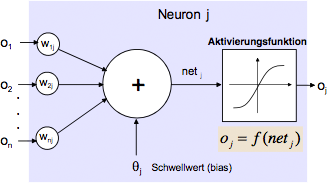
\includegraphics[width=1.1\linewidth]{images/neuron.png}

\[
	net_j = \sum_{i=1}^n o_i \cdot w_{ij} + \Theta_j
\]

Backpropagation - Berechnung des Gewichtsvektor-\textbf{Delta}:

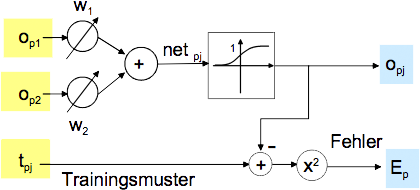
\includegraphics[width=1.1\linewidth]{images/backpropagation.png}

\[
	\Delta w_i = \eta \cdot 2(t_{pj} - o_{pj}) \cdot f'(net_{pj}) \cdot o_{pi}
\]



\newpage

Lorem ipsum dolor sit amet, consectetuer adipiscing elit. Sed
aliquam dolor eu mi. Quisque porttitor. In at tortor. Vestibulum
ante ipsum primis in faucibus orci luctus et ultrices posuere
cubilia Curae; Suspendisse et purus in mauris auctor ullamcorper.
Nunc sed tellus. Donec fringilla egestas magna. Proin arcu libero,
auctor vel, sollicitudin eu, tempus in, orci. Sed pharetra eros ut
nunc. Phasellus congue mauris nec velit. Praesent wisi felis, mollis
non, vehicula nec, porttitor a, ligula. Maecenas dictum aliquet
erat. Ut aliquam, lorem quis convallis molestie, dolor nunc ultrices
arcu, et volutpat dui justo varius ipsum. Vivamus nunc eros,
eleifend a, tincidunt vitae, tristique eget, ante. Ut enim quam,
luctus eu, dictum id, pellentesque sit amet, nulla. Nulla at lectus.
In hac habitasse platea dictumst. Nunc sit amet augue eu leo
vestibulum viverra. Vestibulum quis dui sed quam porttitor
convallis. Nulla vitae magna.

\section{Foo}

Lorem ipsum dolor sit amet, consectetuer adipiscing elit. Sed
aliquam dolor eu mi. Quisque porttitor. In at tortor. Vestibulum
ante ipsum primis in faucibus orci luctus et ultrices posuere
cubilia Curae; Suspendisse et purus in mauris auctor ullamcorper.
Nunc sed tellus. Donec fringilla egestas magna. Proin arcu libero,
auctor vel, sollicitudin eu, tempus in, orci. Sed pharetra eros ut
nunc. Phasellus congue mauris nec velit. Praesent wisi felis, mollis
non, vehicula nec, porttitor a, ligula. Maecenas dictum aliquet
erat. Ut aliquam, lorem quis convallis molestie, dolor nunc ultrices
arcu, et volutpat dui justo varius ipsum. Vivamus nunc eros,
eleifend a, tincidunt vitae, tristique eget, ante. Ut enim quam,
luctus eu, dictum id, pellentesque sit amet, nulla. Nulla at lectus.
In hac habitasse platea dictumst. Nunc sit amet augue eu leo
vestibulum viverra. Vestibulum quis dui sed quam porttitor
convallis. Nulla vitae magna.

\section{Bar}

Lorem ipsum dolor sit amet, consectetuer adipiscing elit. Sed
aliquam dolor eu mi. Quisque porttitor. In at tortor. Vestibulum
ante ipsum primis in faucibus orci luctus et ultrices posuere
cubilia Curae; Suspendisse et purus in mauris auctor ullamcorper.
Nunc sed tellus. Donec fringilla egestas magna. Proin arcu libero,
auctor vel, sollicitudin eu, tempus in, orci. Sed pharetra eros ut
nunc. Phasellus congue mauris nec velit. Praesent wisi felis, mollis
non, vehicula nec, porttitor a, ligula. Maecenas dictum aliquet
erat. Ut aliquam, lorem quis convallis molestie, dolor nunc ultrices
arcu, et volutpat dui justo varius ipsum. Vivamus nunc eros,
eleifend a, tincidunt vitae, tristique eget, ante. Ut enim quam,
luctus eu, dictum id, pellentesque sit amet, nulla. Nulla at lectus.
In hac habitasse platea dictumst. Nunc sit amet augue eu leo
vestibulum viverra. Vestibulum quis dui sed quam porttitor
convallis. Nulla vitae magna.


\section{Baz}

Lorem ipsum dolor sit amet, consectetuer adipiscing elit. Sed
aliquam dolor eu mi. Quisque porttitor. In at tortor. Vestibulum
ante ipsum primis in faucibus orci luctus et ultrices posuere
cubilia Curae; Suspendisse et purus in mauris auctor ullamcorper.
Nunc sed tellus. Donec fringilla egestas magna. Proin arcu libero,
auctor vel, sollicitudin eu, tempus in, orci. Sed pharetra eros ut
nunc. Phasellus congue mauris nec velit. Praesent wisi felis, mollis
non, vehicula nec, porttitor a, ligula. Maecenas dictum aliquet
erat. Ut aliquam, lorem quis convallis molestie, dolor nunc ultrices
arcu, et volutpat dui justo varius ipsum. Vivamus nunc eros,
eleifend a, tincidunt vitae, tristique eget, ante. Ut enim quam,
luctus eu, dictum id, pellentesque sit amet, nulla. Nulla at lectus.
In hac habitasse platea dictumst. Nunc sit amet augue eu leo
vestibulum viverra. Vestibulum quis dui sed quam porttitor
convallis.

\ifUseColumns
	\end{multicols}
\fi

\end{document}

